% FIG ch03-02 three sketches composite (Chinese) — requires codex sketch PNGs
\begin{tikzpicture}[font=\sffamily\small, text=BookInk]
  \node[inner sep=0, anchor=south west] (A) at (0,0.38\linewidth) {%
    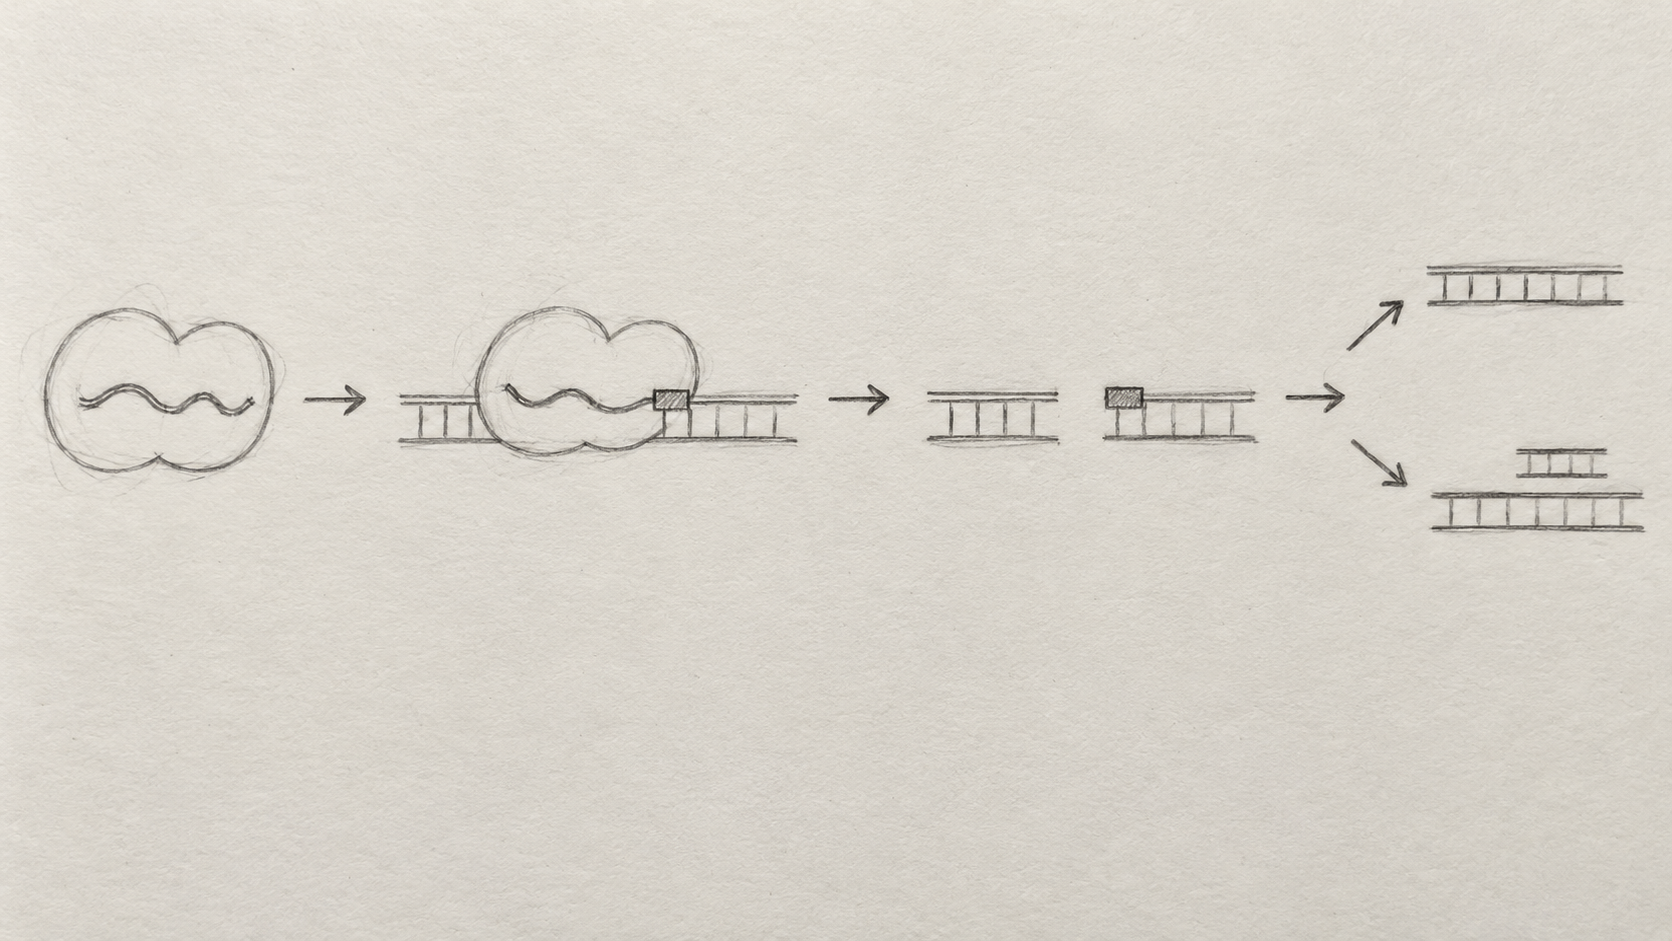
\includegraphics[width=0.32\linewidth]{figures/ch03/ch03-02a-sketch-linear.png}};
  \node[inner sep=0, anchor=south west] (B) at (0.34\linewidth,0.38\linewidth) {%
    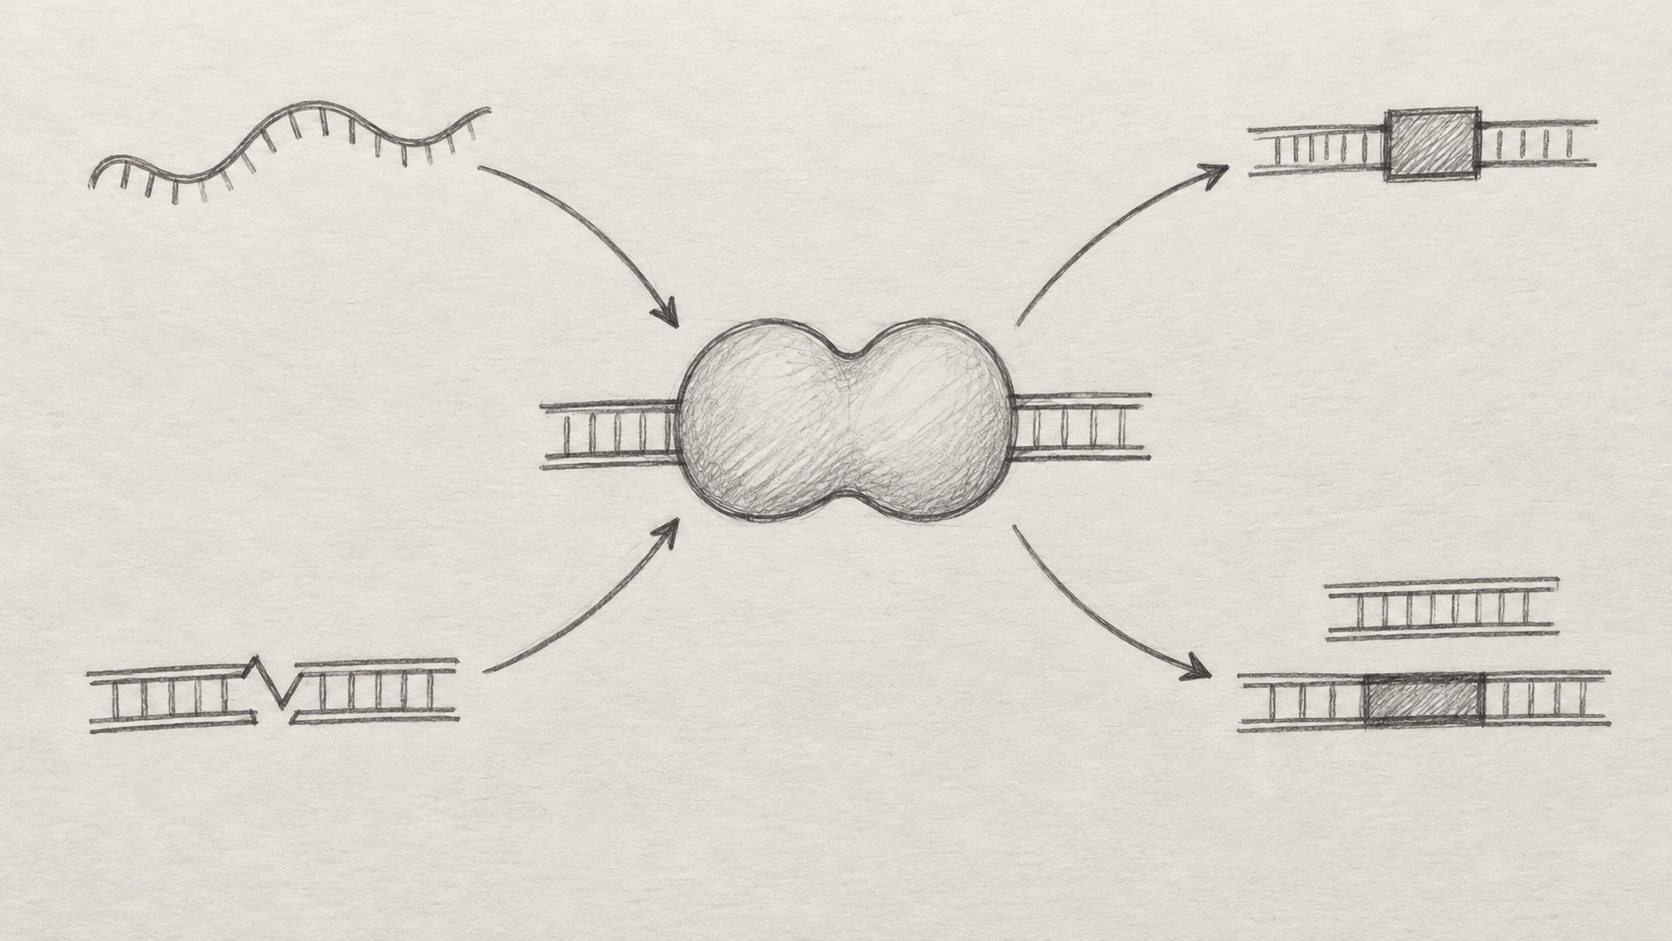
\includegraphics[width=0.32\linewidth]{figures/ch03/ch03-02b-sketch-hub.png}};
  \node[inner sep=0, anchor=south west] (C) at (0.68\linewidth,0.38\linewidth) {%
    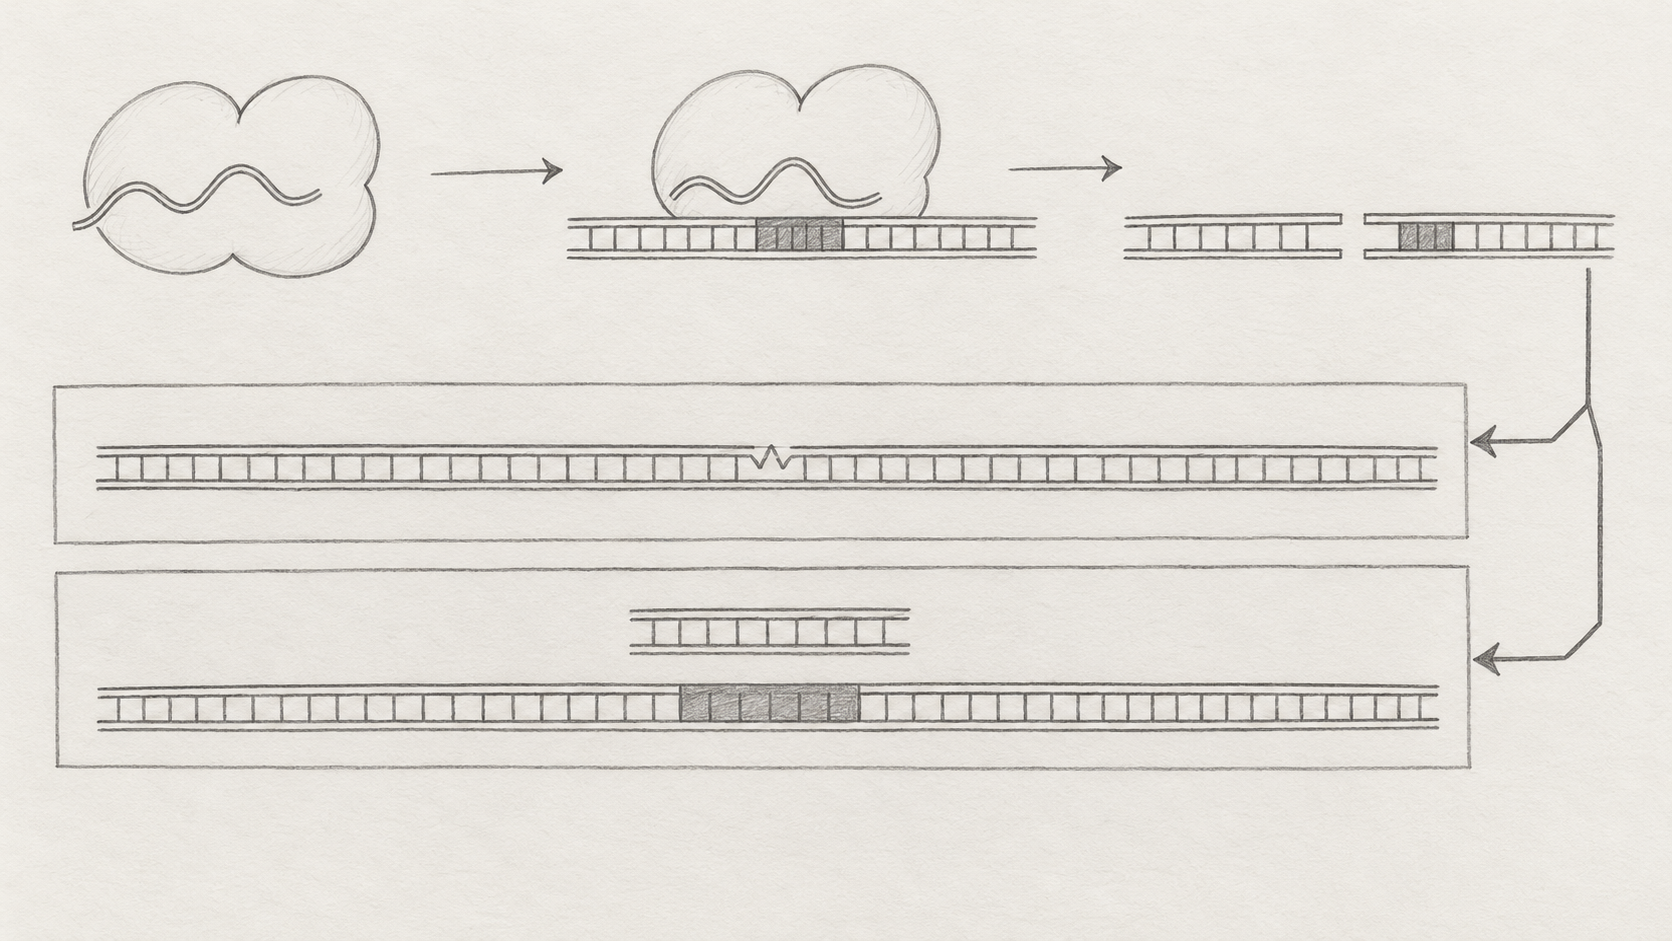
\includegraphics[width=0.32\linewidth]{figures/ch03/ch03-02c-sketch-branch.png}};
  \node[font=\bfseries\Large, anchor=north west] at ($(A.north west)+(2mm,-2mm)$) {A};
  \node[font=\bfseries\Large, anchor=north west] at ($(B.north west)+(2mm,-2mm)$) {B};
  \node[font=\bfseries\Large, anchor=north west] at ($(C.north west)+(2mm,-2mm)$) {C};
  \node[anchor=north, align=center, font=\footnotesize] at (0.16\linewidth,0.34\linewidth)
    {A\quad 线性（左→右）};
  \node[anchor=north, align=center, font=\footnotesize] at (0.50\linewidth,0.34\linewidth)
    {B\quad 中心辐射};
  \node[anchor=north, align=center, font=\footnotesize] at (0.84\linewidth,0.34\linewidth)
    {C\quad 两分支结果};
\end{tikzpicture}
